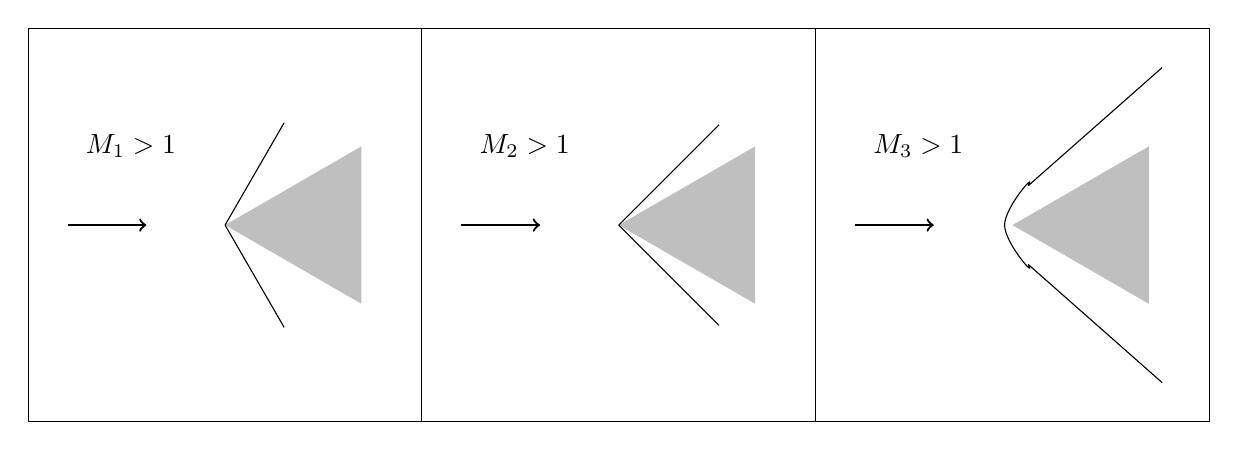
\begin{tikzpicture}
    % Draw the outer rectangle
    \draw (0,0) rectangle (15,5);
    
    % Split the rectangle into three parts
    \draw (5,0) -- (5,5);
    \draw (10,0) -- (10,5);
    
    % First panel: left
    \node[left] at (2.0,3.5) {$M_1 > 1$};
    \draw[->, thick] (0.5,2.5) -- (1.5,2.5);
    \fill[gray!50] (2.5,2.5) -- ++(30:2) -- ++(-90:2) -- cycle;
    \draw (2.5,2.5) -- ++(60:1.5);
    \draw (2.5,2.5) -- ++(-60:1.5);

    % Second panel: middle
    \node[left] at (7.0,3.5) {$M_2 > 1$};
    \draw[->, thick] (5.5,2.5) -- (6.5,2.5);
    \fill[gray!50] (7.5,2.5) -- ++(30:2) -- ++(-90:2) -- cycle;
    \draw (7.5,2.5) -- ++(45:1.8);
    \draw (7.5,2.5) -- ++(-45:1.8);

    % Third panel: right
    \node[left] at (12.0,3.5) {$M_3 > 1$};
    \draw[->, thick] (10.5,2.5) -- (11.5,2.5);
    \fill[gray!50] (12.5,2.5) -- ++(30:2) -- ++(-90:2) -- cycle;
    \draw (12.4,2.5) to[out=+90,in=60] ++(0.3,0.5);
    \draw (12.4,2.5) to[out=-90,in=-60] ++(0.3,-0.5);
    \draw (12.7,3) -- (14.4,4.5);
    \draw (12.7,2) -- (14.4,0.5);
\end{tikzpicture}